%! TeX program = lualatex
\documentclass[12pt,t]{beamer}
\usepackage{graphicx}

% \usepackage{tikz}
% \usetikzlibrary{mindmap,overlay-beamer-styles}
% \usetikzlibrary{shapes.arrows,calc,positioning}%%For arrows
% \usepackage{tikzit}

% \usetikzlibrary{decorations.pathmorphing, backgrounds, shapes, positioning}
% \input{tikz.tikzstyles} % Load styles from the external file
% \input{tikz.tikzdefs} % Load styles from the external file


% \setbeameroption{hide notes}
% \setbeamertemplate{note page}[plain]

% get rid of junk
\usetheme{default}
\beamertemplatenavigationsymbolsempty
\hypersetup{pdfpagemode=UseNone} % don't show bookmarks on initial view

% font
\usepackage{fontspec}
\setsansfont{TeX Gyre Heros}
\setbeamerfont{note page}{family*=pplx,size=\footnotesize} % Palatino for notes

% named colors
\definecolor{offwhite}{RGB}{24,24,24 }
\definecolor{background}{RGB}{226, 218, 218}

\definecolor{title}{RGB}{104, 36, 109}
% \definecolor{title}{RGB}{55, 0, 117}
\definecolor{subtitle}{RGB}{98, 0, 151}

\definecolor{foreground}{RGB}{0, 0, 0}
% \definecolor{hilight}{RGB}{98, 0, 151}
\definecolor{hilight}{RGB}{104, 36, 109}

% \definecolor{gray}{RGB}{193, 18, 31}
\definecolor{gray}{RGB}{104, 36, 109}
\definecolor{vhilight}{RGB}{120, 0, 0}
\definecolor{lolight}{RGB}{155,155,155}
%\definecolor{green}{RGB}{125,250,125}

% use those colors
\setbeamercolor{titlelike}{fg=title}
\setbeamercolor{subtitle}{fg=subtitle}
\setbeamercolor{institute}{fg=hilight}
\setbeamercolor{normal text}{fg=foreground,bg=background}
\setbeamercolor{item}{fg=foreground} % color of bullets
\setbeamercolor{subitem}{fg=gray}
\setbeamercolor{itemize/enumerate subbody}{fg=gray}
\setbeamertemplate{itemize subitem}{{\textendash}}
\setbeamerfont{itemize/enumerate subbody}{size=\footnotesize}
\setbeamerfont{itemize/enumerate subitem}{size=\footnotesize}

% page number
\setbeamertemplate{footline}{%
    \raisebox{5pt}{\makebox[\paperwidth]{\hfill\makebox[20pt]{\color{hilight}
          \scriptsize\insertframenumber}}}\hspace*{5pt}}

% add a bit of space at the top of the notes page
\addtobeamertemplate{note page}{\setlength{\parskip}{12pt}}

% a few macros
\newcommand{\bi}{\begin{itemize}}
\newcommand{\ei}{\end{itemize}}
\newcommand{\ig}{\includegraphics}
\newcommand{\subt}[1]{{\footnotesize \color{subtitle} {#1}}}

% title info
\title{{\Huge Git your sheet together} \\ Git for mathematical writing}
% \subtitle{A researcher's perspective}
\author{\href{http://lchiarini.com}{Leandro Chiarini}}
\institute{Durham University}
\date{\today \\
	\vspace{2em}
}


\begin{document}

% title slide
{
\setbeamertemplate{footline}{} % no page number here
\frame{ \titlepage
   } }

\begin{frame}{Why Version Control?}
	\pause
	This for instance is version control
		%
		\begin{figure}[ht]
		    \centering
		    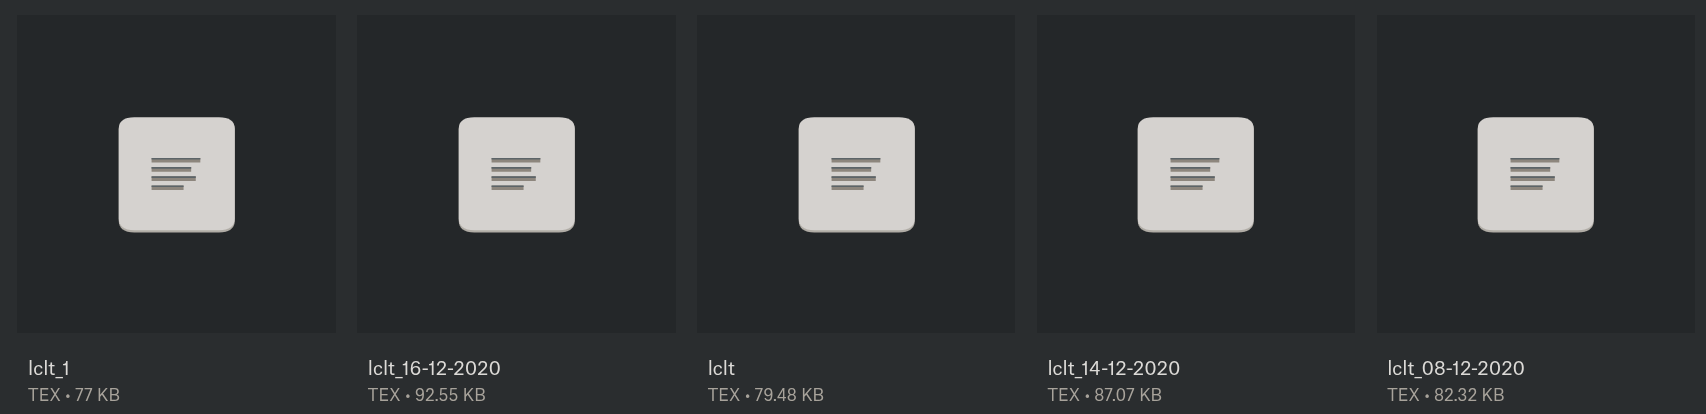
\includegraphics[width=0.6\textwidth]{figs/ScreenShot-without-git.png}
		\end{figure}
		%
		\pause

	But, we can do better
\begin{itemize}
		\pause
    \item Track changes in your work over time
		\pause
    \item Collaborate effectively with co-authors
		\pause
    \item Revert mistakes and explore new ideas without ruining the file structure
\end{itemize}
\end{frame}

\begin{frame}{What is Git?}
\begin{itemize}
    \item A distributed version control system
		\vspace{1em}
		\pause
    \item Records snapshots of your project
		\vspace{1em}
		\pause
    \item Lets you experiment safely
		\vspace{1em}
		\pause
    \item Works especially well with plain text formats like \LaTeX
		\pause 
		\vspace{.5em}
		\begin{itemize}
			\item To save all your photos, better use something else.
		\end{itemize}
		
\end{itemize}
\end{frame}

\begin{frame}{Key Concepts}
\begin{itemize}
    \item Repository (repo)
		\pause
    \item Commit and staging area
		\pause
    \item Branches and merging
		\pause
    \item Remote vs local
\end{itemize}
\end{frame}

\begin{frame}{Basic Workflow}
\begin{itemize}
    \item \texttt{git init} --- start a new repo
		\pause
    \item \texttt{git add file.tex} --- stage changes
		\pause
    \item \texttt{git commit -m "Message"} --- save changes
		\pause
    \item \texttt{git log}, \texttt{git status}, \texttt{git diff}
\end{itemize}
\end{frame}

\begin{frame}{Git with Remote Repositories}
\begin{itemize}
    \item \texttt{git clone <url>}
		\pause
    \item \texttt{git push} and \texttt{git pull}
		\pause
    \item Hosting options: GitHub, GitLab, Bitbucket
		\pause
    \item Manage collaboration through remotes
\end{itemize}
\end{frame}

\begin{frame}{Undo Without Fear}
\begin{itemize}
    \item Revert to any point in history
		\pause
    \item Branch to test new proof strategies
		\pause
    \item Use \texttt{stash} to temporarily save changes
		\pause
    \item Git makes experimenting safe!
		\pause
\end{itemize}
\end{frame}

\begin{frame}{Branches for Experiments}
\begin{itemize}
    \item Try out changes on separate branches
		\pause
    \item Merge back once satisfied
		\pause
    \item Keep main branch stable
		\pause
    \item Resolve merge conflicts with care
\end{itemize}
\end{frame}

\begin{frame}{Best Practices for \LaTeX}
\begin{itemize}
    \item Use one sentence per line
		\pause
    \item Ignore build files with \texttt{.gitignore}
		\pause
    \item Commit logically grouped changes
		\pause
    \item Write meaningful commit messages
\end{itemize}
\end{frame}

\begin{frame}{Collaborating with Git}
\begin{itemize}
    \item Pull requests (PRs) for review
		\pause
    \item Review diffs of mathematical arguments
		\pause
    \item Assign co-author responsibilities
		\pause
    \item Use comments to discuss changes
\end{itemize}
\end{frame}

\begin{frame}{Tooling and Interfaces}
\begin{itemize}
    \item GitHub Desktop, GitKraken, SourceTree
		\pause
    \item Overleaf Git integration
		\pause
    \item VS Code with Git support
		\pause
    \item Diff tools: \texttt{latexdiff}, \texttt{diffpdf}
\end{itemize}
\end{frame}

\begin{frame}{Practical Exercise}
\begin{itemize}
    \item Initialise a repo for a paper
		\pause
    \item Make edits and commit
		\pause
    \item Create and merge a branch
		\pause
    \item View commit history
\end{itemize}
\end{frame}

\begin{frame}{Key Takeaways}
\begin{itemize}
    \item Git = powerful safety net
		\pause
    \item Track your mathematical thought process
		\pause
    \item Collaborate cleanly and confidently
		\pause
    \item Undo without fear
\end{itemize}
\end{frame}


\end{document}
